If solution exists for the given system of linear equations 
then they are said to be consistent, otherwise they are inconsistent. we can represent the given lines in the form of
\begin{align}
\myvec{1&3}\vec{x} = 5\\
\myvec{2&6}\vec{x} = 8
\end{align}
writing the above equations in matrix form
\begin{align}
\myvec{1 & 3 & -5 \\ 2 & 6 & -8}\vec{x} = 0
\end{align}\\
The matrix equation is row reduced as follows
\begin{align}
\myvec{1 & 3 & -5 \\ 2 & 6 & -8}  \xleftrightarrow[]{R_2\leftarrow R_2-2R_1} \myvec{1 & 3 & -5 \\ 0 & 0 & 2}
\end{align}\\
Thus, from the above row reduced form we can conclude that the given system of lines has no solution. Therefore, they are inconsistent.  See \ref{Fig 0:solutions/det/54/}
\begin{figure}
\centering
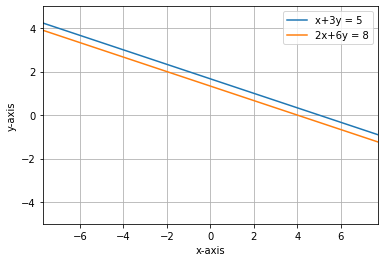
\includegraphics[width=\columnwidth]{./solutions/det/54/assignment2.png}
\caption{Plot showing the given two lines are parallel}
\label{Fig 0:solutions/det/54/}
\end{figure}
